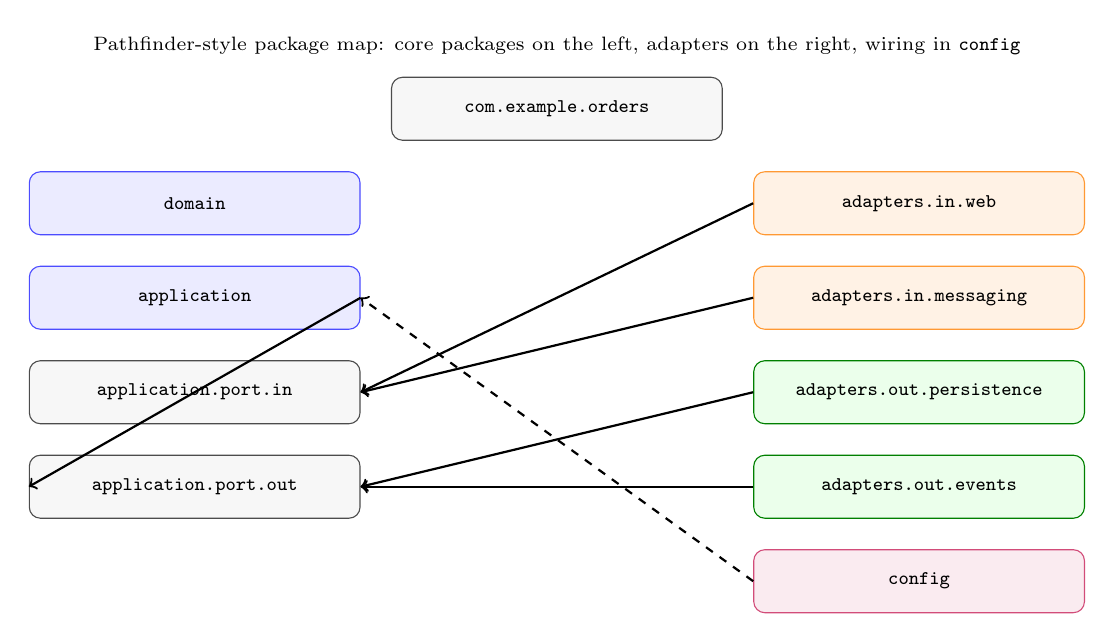
\begin{tikzpicture}[
    folder/.style={rectangle, draw=black!70, rounded corners, minimum width=4.2cm, minimum height=0.8cm, align=left, font=\scriptsize, fill=gray!6},
    core/.style={rectangle, draw=blue!70, rounded corners, minimum width=4.2cm, minimum height=0.8cm, align=left, font=\scriptsize, fill=blue!8},
    adapterIn/.style={rectangle, draw=orange!80, rounded corners, minimum width=4.2cm, minimum height=0.8cm, align=left, font=\scriptsize, fill=orange!10},
    adapterOut/.style={rectangle, draw=green!50!black, rounded corners, minimum width=4.2cm, minimum height=0.8cm, align=left, font=\scriptsize, fill=green!8},
    cfg/.style={rectangle, draw=purple!70, rounded corners, minimum width=4.2cm, minimum height=0.8cm, align=left, font=\scriptsize, fill=purple!8}
]
    \node[folder] (root) at (0,3.6) {\texttt{com.example.orders}};

    \node[core] (domain) at (-4.6,2.4) {\texttt{domain}};
    \node[core] (application) at (-4.6,1.2) {\texttt{application}};
    \node[folder] (appIn) at (-4.6,0.0) {\texttt{application.port.in}};
    \node[folder] (appOut) at (-4.6,-1.2) {\texttt{application.port.out}};

    \node[adapterIn] (inweb) at (4.6,2.4) {\texttt{adapters.in.web}};
    \node[adapterIn] (inmsg) at (4.6,1.2) {\texttt{adapters.in.messaging}};
    \node[adapterOut] (outdb) at (4.6,0.0) {\texttt{adapters.out.persistence}};
    \node[adapterOut] (outevt) at (4.6,-1.2) {\texttt{adapters.out.events}};
    \node[cfg] (config) at (4.6,-2.4) {\texttt{config}};

    \draw[->, thick] (inweb.west) -- (appIn.east);
    \draw[->, thick] (inmsg.west) -- (appIn.east);
    \draw[->, thick] (application.east) -- (appOut.west);
    \draw[->, thick] (outdb.west) -- (appOut.east);
    \draw[->, thick] (outevt.west) -- (appOut.east);

    \draw[->, thick, dashed] (config.west) -- (application.east);
    \node[font=\scriptsize, align=center] at (0,4.4) {Pathfinder-style package map: core packages on the left, adapters on the right, wiring in \texttt{config}};
\end{tikzpicture}
